\chapter{Methods}\label{methods}

\section{Introduction}
Since its introduction \parencite{aertsenSpectrotemporalReceptiveFields1980a}, the spectro-temporal receptive field (STRF) has been a widely used method for studying auditory neurons. Nevertheless, it has been shown STRF does not manage to capture nonlinearlities in neuronal activity. Therefore, my thesis will attempt to apply a convolutional neural network architecture on calcium imaging data, which will then be linearized to an interpretable DSTRF, as described by \textcite{keshishianEstimatingInterpretingNonlinear2020}. 
The data used in this project consists of calcium imaging data, where a genetically encoded calcium indicator (GECI) has been expressed in auditory cortex neurons of mice. This indicator has fluorescent properties, and thus intraneuronal calcium dynamics can be recorded using widefield imaging.

\section{Experimental setup, data description and preprocessing}
As for the experimental setup, the neural representation of random tone sequences in mice \qst{(CBA/JRj, female, age: 2-3 months, n=10)} was investigated. The mice were locally transfected the calcium indicator jGCaMP8m (described below) and the whole auditory cortex was chronically imaged (1p widefield, 100 Hz). Imaging was performed through a cranial window (ø=3.0-4.2 mm) centered above the AC starting after 2-3 weeks of viral expression.

Each trial lasts for 4.2 seconds, at a recording frequency of 100 Hz. Therefore, 420 frames of video were colected, at a resolution of 304 $\times$ 340 pixels.

The raw data collected from the animals was preprocessed using the Controller software developed within the lab. The standard preprocessing methods have been used: motion correction, deconvolution and denoising of the calcium imaging. The resulting frames of resolution 152x170 were further used as input to the convolutional neural network.

\subsection{Calcium imaging}
The calcium indicator that was used is jGCaMP8m. The jGCaMP8m indicator is part of the GCaMP family, and show improved kinetics compared to previous versions, without compormising sensitivity or brightness \parencite{zhangFastSensitiveGCaMP2023}. Additonally, this indicator can track neurons with spike rates up to 50 Hz, and are also more linear in their fluorescence, allowing for more robust deconvolution during spike extraction \parencite{zhangFastSensitiveGCaMP2023}.

Calcium imaging is an indirect indicator of neural activity, due to the important role of calcium ions $\mathrm{Ca}^{2+}$ as intracellular messengers in mammals \parencite{grienbergerImagingCalciumNeurons2012}. Only free calcium ions are biologically active \parencite{grienbergerImagingCalciumNeurons2012}. The dominant determining factor are voltage-gated calcium channels (VGCCs), which represent a broad class of channels which are highly selective for calcium ions and exhibit a large range of voltage-dependent behaviours.

The jGCaMP8m calcium indicator works similarly to other indicators in the GCaMP family, being a single-fluorophore GECI. GCaMPs in general consist of three elements: a circularly permuted enhanced green fluorescent protein (EGFP), the calcium binding protein calmodulin, and the calmodulin-binding peptide M13. The EGFP is flanked on both sides by the other two components. In the presence of calcium, the flueoresence of the indicator increases, giving a visual indication of concentration of calcium and, therefore, of the neural activity \parencite{grienbergerImagingCalciumNeurons2012}.

\begin{figure}[ht]
	\centering
	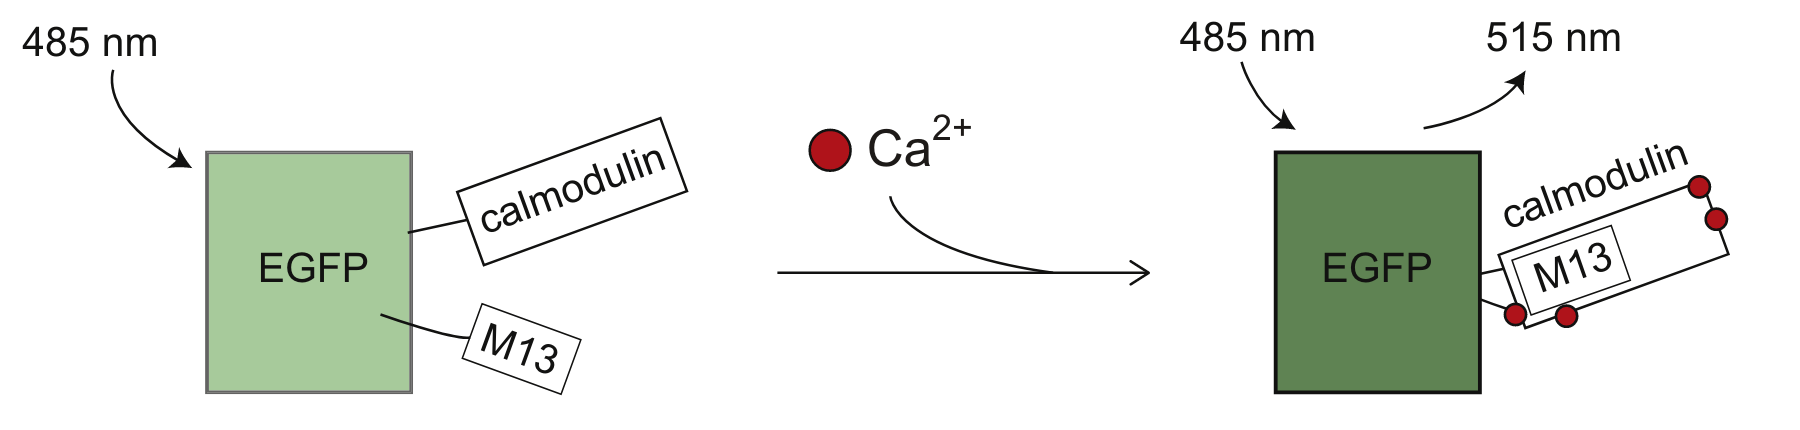
\includegraphics[scale=0.3]{gcamp}
	\caption{\parencite{grienbergerImagingCalciumNeurons2012}}
\end{figure}



\section{Stimulus}
\qst{The dynamic random chord (DRC) stimulus has been used during imaging, in order to elicit a response in the auditory cortex. The stimulus consists of a sequence of chords of random frequency. A chord contains one or more identically loud tones of various frequencies, played simultaneously. Two chord are played per trial, each with a duration of 0,05 s = 50 ms and a silent interval of 50 ms between successive chords. The trial ends 2,05 seconds after the end of the last chord, and the next trial commences immediately with 2 seconds start delay before the first chord of that trial is played.}

The stimulus is converted into a spectrogram using the fast Fourier transform. Initially, the frequencies are binned into intervals and displayed along the y-axis, while the 220 time samples (counted from stimulus onset) are displayed along the x-axis. The spectrogram below is a concrete example, showcasing the stimulus spectrogram from mouse 219, recording 25, trial 1:

\begin{figure}[ht]
\centering
	\includegraphics[scale=0.5]{example_spec_mouse219r25}
\caption{The spectrogram above shows an example of the DRC stimulus used for our experiments. The time in seconds is shown on the x-axis and the frequency bin on the y-axis, respectively. The two chords played in this trial can be clearly seen on the left of the figure.}
\end{figure}

Moreover, the analysis is conducted using the DSTRF python implementation provided by the authors of the original paper (\href{https://github.com/naplab/DSTRF}{https://github.com/naplab/DSTRF}). The described CNN network is trained to predict the activity of each pixel, when given the audio spectrogram of the auditory stimulus as input. Then, as detailed in the original paper, as well as below, this network is linearized in order to extract the interpretable DSTRF.

\section{Convolutional neural networks}

A convolutional neural network is a type of neural network inspired by visual perception \parencite{liSurveyConvolutionalNeural2022}. As opposed to multilayer perceptrons, these networks take into consideration the spatial layout of the data by enforcing local connections \parencite{zhangDiveDeepLearning2024}. An optimizer is used in order to minimize the loss function, which models the error of the predicted output compared to the actual output \parencite{liSurveyConvolutionalNeural2022}. Concretely applied to the application presented in this thesis, the input of the network consists of individual pixels of the preprocessed image. When given the recorded calcium traces as indication of the correct output during the training session, the neural network optimizes the weights so that it approximates the activity as well as possible. 
	
The architecture described by \textcite{keshishianEstimatingInterpretingNonlinear2020} is used. This architecture consists of two types of layers: convolutional and fully connected layers. Convolutional layers apply a cross-correlation operation on the layer input by means of a kernel. The equation describing this operation is as follows adapted from \textcite{zhangDiveDeepLearning2024}\:

\begin{equation}
	H_{i, j, d} = \sum_{a=-\Delta}^\Delta \sum_{b=-\Delta}^\Delta \sum_c V_{a, b, c ,d} X_{i+a, j+b, c}
\end{equation}

A convolutional layer consists of the input $X$ (height x width x channels), an output $H$ (height x width x number of feature maps) and a  set of $c$ kernels (weights) for each feature map. The obtained feature maps represent different aspects of the input data, corresponding to the weights used \parencite{liSurveyConvolutionalNeural2022}.

%On the other hand, fully connected layers are used in the final layers of a CNN network in order to achieve a global perspective on the input image and introduce non-local dependencies.

In order to reach arrive at an interpretable solution, linearization of the resulting network is used. Assuming that the network uses the ReLU activation function, the resulting weight $w_{path}$ for any path from an input node to the output node can be calculated by multiplying the weights $w_l$ across all layers $l$. A more detailed explanation is given below.

\begin{proof}[Explanation]
Assume a valid path $p$ generated by selecting one node $n_{li}$ per layer $l$, where $i \in \{1, s_l\}$ and $s_l$ is the number of neurons in each layer. $s_l$ might differ for each layer, depending on the architecture. The number of total paths corresponding to one input is:

\begin{equation}
	t_{in} = \prod_{l=1}^n s_l
\end{equation} 

The weight obtained from one path can be expressed as such:

\begin{equation}
	w_{in, p} = \prod_{l=1}^{n} w_{l}
\end{equation}
, where $p$ indexes all possible paths from input node $in$, therefore $p \in \{1, t_{in}\}$

Moreover, for each path starting from the same input node, it is possible to further multiply the obtained weights in order to get a single weight corresponding to each input node.

\begin{equation}
	w_{in} = \sum_p w_{in, p}
\end{equation}

\end{proof}

\begin{figure}[ht]
	\centering
	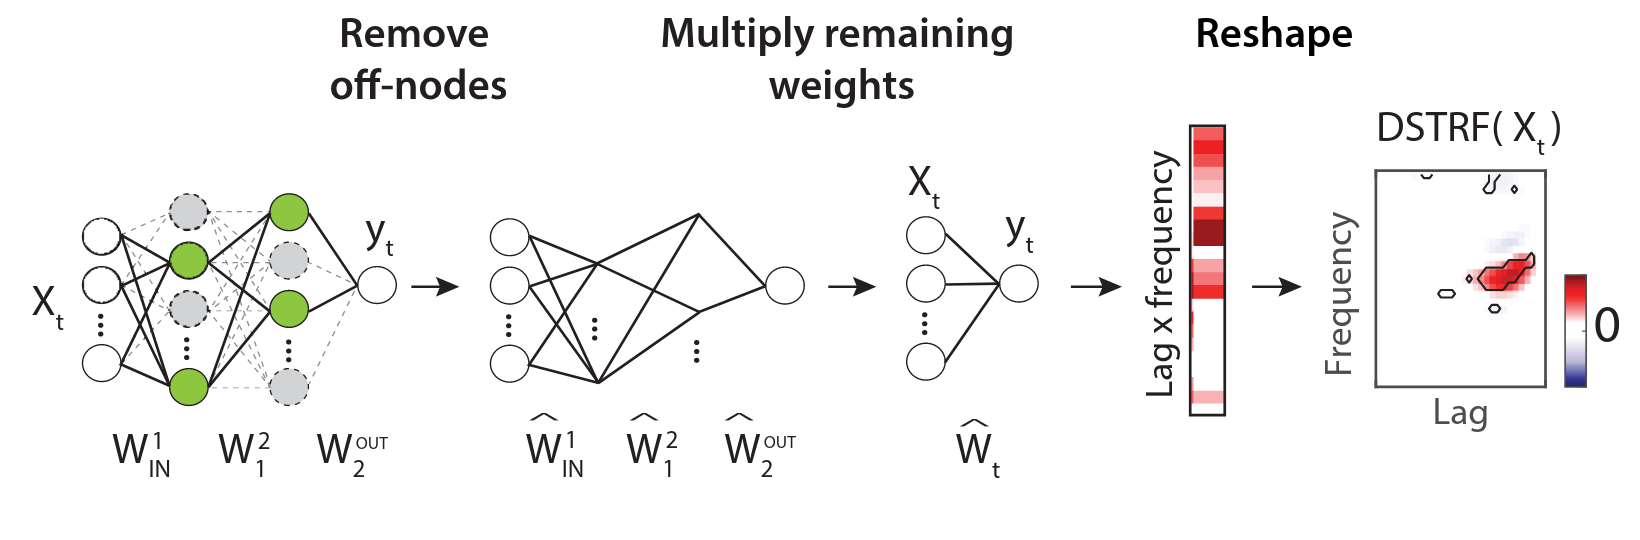
\includegraphics[scale=0.3]{linearization}
	\caption{\parencite{keshishianEstimatingInterpretingNonlinear2020}}
\end{figure}

The resulting weight matrix $\mnot{w}$ contains one weight for each input (i.e spectrogram bin), which can be visualized as the DSTRF for that particular window of the stimulus.

\section{Mouse auditory system}
The brain region targeted by the calcium imaging is the auditory cortex. The murine auditory cortex represents the site of termination of medial geniculate body (MG) ascending fibers \parencite{malmiercaAuditorySystem2012}. The auditory cortex is classified into five auditory fields based on characteristics of their auditory response. Two out of five regions are tonotopically organized: the primary auditory field (AI) and the anterior auditory field (AAF) \parencite{malmiercaAuditorySystem2012}.

The mouse auditory system has some general features in common with that of humans \parencite{malmiercaAuditorySystem2012}. Its comparatively small size and advances in gene targeting techniques has made the mouse a widely used model in auditory research \parencite{malmiercaAuditorySystem2012}. In the primary auditory cortex (A1), a tonotopic organization of the cortex has been discovered  \parencite{malmiercaAuditorySystem2012}. The tonotopy of the cochlea, where sound waves are transduced into electrical signals, persists thoroughout the brainstem. More specifically, the auditory pathway consisting of the cochlea, the cochlear nucleus, the superior olivary complex, the inferior colliculus, the medial geniculate body and finally, the auditory cortex all exhibit tonotopic properties  \parencite{malmiercaAuditorySystem2012}.

The sound waves propagate through and mechanically through the outer and middle ear \parencite{malmiercaAuditorySystem2012}. In the inner ear, they are transduced into electrical signals by hair cells, which travel through the cochlear nerve until they reach the brainstem, where they undergo obligatory synaptic interruption in the cochlear nucleus. Individual fibers ramify and ascend through a number of parallel tracts, converging into the auditory midbrain and inferior colliculus (IC). These converged fibers synapse in the medial geniculate body (MG), which finally relays the signals to the auditory cortex \parencite{malmiercaAuditorySystem2012}.

Therefore, in order to estimate the input to the cortical auditory neurons as well as possible, a model of early processing encompassing all previous brain structures will be used in an attempt to maximize the potential of the neural network. A model by \textcite{yangAuditoryRepresentationsAcoustic1992} plays this role in the original paper. Due to time constraints, an already available model was used, as opposed to designing one from scratch.

\todo{simple figure of auditory system}

\section{Dynamic STRF}
Referencing the models presented in the Background section, the DSTRF is an estimation method of the filter $\mnot{k}$. The novelty of DSTRF comes from the fact that it attempts to compute a different filter $\mnot{k_{sample}}$ for each subsequent sample of neural activity. In the case of this paper, given the $n = 220$ frames collected after the onset of the stimulus, 220 different filters ($\mnot{k_1}, \mnot{k_2}, \mnot{k_3}, \dots, \mnot{k_n}$) will be computed and concatenated into a movie across the temporal dimension. 

A network consisting of nodes implementing the ReLU activation function is a universal approximator, which holds for all multilayer feedforward neural networks in general \parencite{hornikMultilayerFeedforwardNetworks1989}. The architecture used to analyse the data is both multilayer, since it contains multiple layer that are connected such that one layer's output is the next layer's input, and also feedforward, since each connection only connects one layer to the next, without any feedback or recursive connection to itself or the previous layers. Moreover, the ReLU activation functions allows the network to approximate any function through piecewise line segments \parencite{keshishianEstimatingInterpretingNonlinear2020}. Using the linearlization process discussed above, we can obtain a weight vector of the same size as the network input, which can considered a filter $\mnot{k}$. Therefore, the stimulus (input of the network) can be multiplied with this filter to get the response estimation $\hat{r} = \mnot{k^T}\mnot{s}(t)$, acting in a similar fashion to STRF.

\begin{figure}[ht]
	\centering
	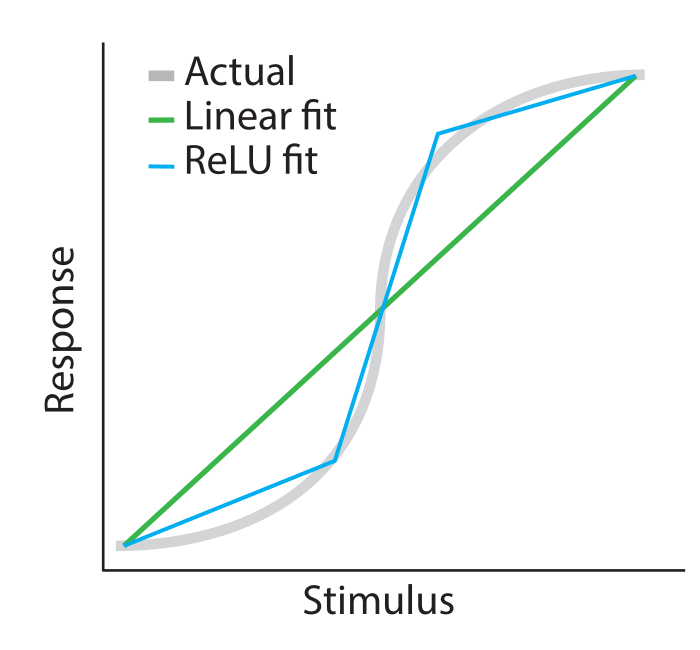
\includegraphics[scale=0.4]{relu}
	\caption{\parencite{keshishianEstimatingInterpretingNonlinear2020}}
\end{figure}

\subsection{CNN network}
The architecture we used is the original implementation in \parencite{keshishianEstimatingInterpretingNonlinear2020}. This architecture closely follows the CNN architectural principles, consisting of a feature extraction network and a feature summation layer. The networks takes the $T \times F$ bins of the stimulus spectrogram as as input, and outputs the estimated response $\hat{r_i}$ for all $H \times W$ pixels of the image. During the training process, this response is compared to the real recorded response $r_i$. Then, the loss function is computed and the weights of the network are optimized by backpropagation.

\begin{figure}[ht]
	\centering
	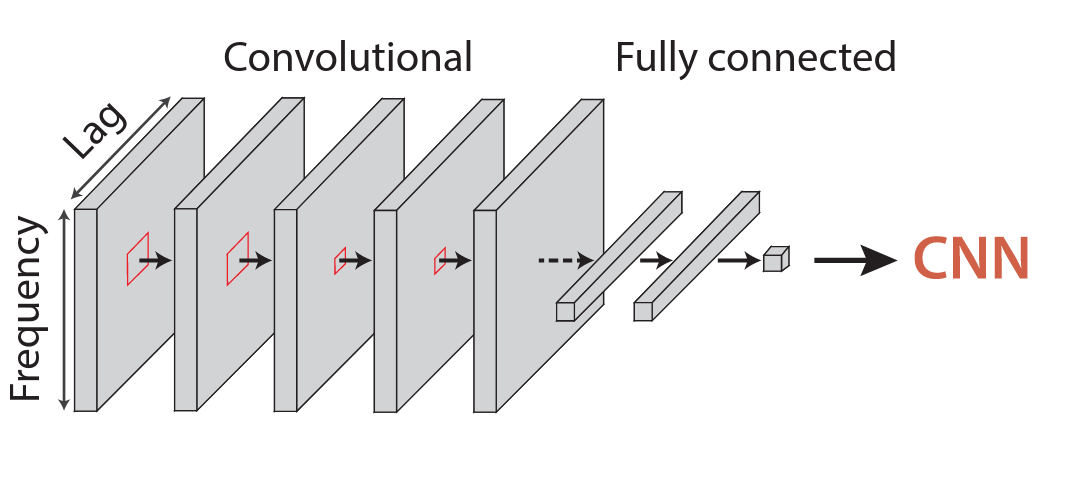
\includegraphics[scale=0.4]{CNN_arch}
	\caption{\parencite{keshishianEstimatingInterpretingNonlinear2020}}
\end{figure}

The feature extraction component of the network is comprised of three consecutive convolutional layers with eight kernel size of $3 \times 3$ each, one layer with four $1 \times 1 1$ kernels, and one layer with one $1 \times 1$ kernel. The first layer produces 8 feature maps of size $168 \times 150$, which are then stacked and provided as input to the next layer. The output of the first three layers is of shape $164 \times 146 \times 8$, which is drastically dimensionally reduced through the following layer to $164 \times 146 \times 4$, since only four kernels are used. Then, the latent representation is reduced further to $164 \times 146 \times 1$.

The feature summation layers contains two layer of 32 nodes each. In the feature summation layer, the input is first flattened into a vector in order to be properly sized as input to the fully connected layers. Therefore, the $164 \times 146$ feature maps becomes an $N = 164 * 146 = 23944$-size vector. This vector $v$ is processed through 2 fully connected layers, $l_1$ and $l_2$, such that:

\begin{align}
	l_1 &= \sum_{i=1}^N w_1i x_i = \mnot{w_1^T}\mnot{x} \\
	l_2 &= \sum_{j=1}^N w_2j l_{1_j} = \mnot{w_2^T}\mnot{l_1} = \mnot{w_2^T}\mnot{w_1^T}\mnot{x}
\end{align}

The output $\hat{r}$ is a scalar representing the neural activity (calcium activation) at a particular time $t$, as derived from the input spectrogram windows starting at $t - t_{delay}$ and ending at time $t$.

The hyperparameters of this network (number of convolutions l layers, number of fully connected layers, kernel size, number of nodes etc.) were found by the authors by optimizing the prediction accuracy on their own dataset.

The loss function used by \parencite{keshishianEstimatingInterpretingNonlinear2020} is a linear combination of MSE and Pearson's coefficient:

\begin{align}
	MSE &= \sum_i (\hat{r_i} -r_i)^2 \\
	PCC &= \frac{\sum _i (r - \overline{r}) (\hat{r} - \overline{r})}{\sqrt{\sum _i (r - \overline{r})^2 \sum _i (\hat{r} - \overline{r})^2}} \\
	\mathcal{L} &= \frac{1}{n} \sum_i (\hat{r_i} -r_i)^2 - \frac{\sum _i (r - \overline{r}) (\hat{r} - \overline{r})}{\sqrt{\sum _i (r - \overline{r})^2 \sum _i (\hat{r} - \overline{r})^2}}
\end{align}

In order to linearize the network, it it easier to convert the 2D CNN architecture to a 1D fully connected MLP architecture. This is possible, since the CNN architecture applies the same weights while convoluting over the input using the kernel, while the fully connected architecture uses unique (and thus more) weights. In other words, the conversion process consists of expanding the implicit repetition of weights represented by the kernel into an explicit list where weights are not unique, but repeating. This procedure is likewise presented by \textcite{keshishianEstimatingInterpretingNonlinear2020}, and will be reproduced here.

Given the all zeros weight tensor $W$ with dimensions $M \times N \times C \times M \times N \times L$, where M, N, C are the dimensions of input to the convolutional layer (rows, columns, channels (depth)), L is the number of kernels in a layer, where each kernel $K_l$ is of dimensions $H \times W \times C$, we can populate tensor $W$ by filling in the below equation for every value of $m$, $n$, and $l$:

\begin{equation}
	W\left[m - \left\lfloor\frac{H}{2}\right\rfloor:m+ \left\lfloor\frac{H}{2}\right\rfloor, n- \left\lfloor\frac{W}{2}\right\rfloor:n+ \left\lfloor\frac{W}{2}\right\rfloor, 1:C; m, n, l\right] = K_l
\end{equation} 
\noindent , where $:$ represents the slicing operator, $a:b \leftrightarrow \forall i \in \{a, b\}, i \in \mathbb{Z}, a, b \in \mathbb{Z}$

To explain verbally, taking a $3 \times 3 \times 8$ kernel $k$ as an example, the formula explicitly copies the kernel weights across each $3 \times 3 \times 8$ area of the input where it was applied, in order to assign a weight to each input node and remove the need of convolution or "sliding" of the kernel across the input.

Assuming the use of the ReLU activation function and the absence of bias, the linearization procedure described above can be used.

\subsection{Hyperparameter optimization}
\todo{to write}

\subsection{Jackknifing and cross-validation}
During the training process, \emph{cross-validation} was used. Cross-validation is an established method in the statistical and machine learning community, and it used to estimate prediction error \parencite{batesCrossValidationWhatDoes2024}. Cross-validation consists of splitting $n$ samples  into a training subsample (size $n-1$) and a validation subsample (size $1$) in all $n$ possible ways \parencite{stoneCrossValidatoryChoiceAssessment1974}.  While using a single split amounts to validation, averaging results over multiple splits represents cross-validation \parencite{arlotSurveyCrossvalidationProcedures2010}. The exhaustive leave-one-out cross validation is defined as:

\begin{equation}
	\hat{\mathcal{L}}^{\mathrm{LOO}}(A; D_n) = \frac{1}{n} \sum_{j=1}^n \gamma \left( A \left( D^{(-j)}_n \right); \xi_j \right)
\end{equation}
\todo{explanation of formula}

In the original paper by \textcite{keshishianEstimatingInterpretingNonlinear2020}, \emph{jackknifing} was used in order to ensure that the obtained DSTRF coefficients are statistically significant. To that end, 20 CNNs were trained, leaving out disjoint 1/20 portions of the data for each network. Therefore, a distribution of samples was obtained for each coefficient. If 19 of 20 samples agree on the sign of a certain coefficient, then the value is considered significant ($p=0.05$) and the mean of the samples is taken as the final coefficient. In case of insignificance, the coefficient is set to 0 \parencite{keshishianEstimatingInterpretingNonlinear2020}.

\section{Code implementation}

\section{Conclusion}
In conclusion, calcium imaging is used to record and collect data from the mouse auditory cortex. The fluorescence of the GCaMP indicator correlates with neuronal activity. The obtained recordings are then used as labels to train a convolutional neural network to predict neuronal activity from the perceived auditory stimulus. The trained network is then linearized in order to obtain the direct weights corresponding to each input node (image pixel). These weights represent the DSTRF of that particular pixel at a specific time point. By concatenating the DSTRFs obtained for different time points, a chronological video can be obtained for each pixel.